\documentclass{standalone}
\usepackage{tikz}

\begin{document}

    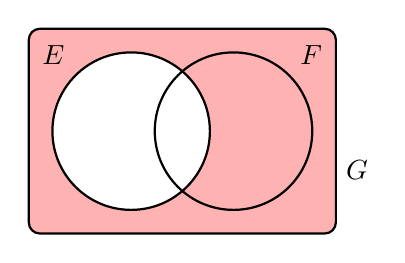
\begin{tikzpicture}[baseline=(current bounding box.center), thick, set/.style = {circle, minimum size = 2cm, fill=red!30}]

        \filldraw[rounded corners, fill=red!30, draw=black] (-1.3, -1.3) rectangle (2.6, 1.3) {};
        \node[set,label={135:$E$}] (A) at (0,0) {};
        \node[set,label={45:$F$}] (B) at (1.3,0) {};
        \node[right] at (2.6, -.5) {$G$};

        \begin{scope}
            \clip (0,0) circle(1cm);
            \fill[white](0,0) circle(1cm);
        \end{scope}

        \draw (0,0) circle(1cm);
        \draw (1.3,0) circle(1cm);

    \end{tikzpicture}

\end{document}